% !TeX program = xelatex
\documentclass[UTF8,fontset=fandol,10pt]{ctexart}
\usepackage[a3paper,portrait,margin=11mm]{geometry}
\usepackage{amsmath,amssymb,bm,graphicx,booktabs,array,xcolor}
\usepackage{newtxtext,newtxmath}
\usepackage{microtype}
\usepackage{fix-cm}
\usepackage[colorlinks=true,urlcolor=teal]{hyperref}
\definecolor{navy}{HTML}{152C46}
\definecolor{teal}{HTML}{007C83}
\definecolor{muted}{HTML}{526171}
\definecolor{pale}{HTML}{EAF4F3}
\definecolor{line}{HTML}{CFD8E0}
\pagestyle{empty}
\linespread{1.0}
\setlength{\parindent}{0pt}
\setlength{\parskip}{2pt}
\setlength{\abovedisplayskip}{2pt}
\setlength{\belowdisplayskip}{2pt}
\setlength{\abovedisplayshortskip}{2pt}
\setlength{\belowdisplayshortskip}{2pt}
\newcommand{\sect}[2]{\par\vspace{2pt}{\color{teal}\bfseries\fontsize{13.5}{16}\selectfont #1\quad #2}\par\vspace{1pt}{\color{line}\hrule}\vspace{2pt}}
\newcommand{\subhead}[1]{\par\vspace{2pt}{\bfseries\color{navy}#1}\par}
\newcommand{\smallnote}[1]{{\fontsize{8.6}{10.7}\selectfont\color{muted}#1\par}}
\newcommand{\takeaway}[1]{\par\vspace{3pt}\colorbox{pale}{\parbox{\dimexpr\linewidth-2\fboxsep}{\bfseries\color{teal}#1}}\par}
\newcommand{\posterheader}[3]{\colorbox{navy}{\parbox{\dimexpr\textwidth-2\fboxsep}{\vspace{5mm}\hspace{3mm}\begin{minipage}{\dimexpr\linewidth-6mm}\color{white}{\bfseries\fontsize{24}{27}\selectfont #1\par}\vspace{2mm}{\fontsize{11}{14}\selectfont #2\hfill #3}\end{minipage}\vspace{5mm}}}\par\vspace{4mm}}
\newcommand{\columnstart}{\begin{minipage}[t]{0.318\textwidth}\vspace{0pt}}
\newcommand{\columnend}{\end{minipage}}
\newcommand{\colsep}{\hfill}
\newcommand{\posterfooter}[1]{\par\vspace{3mm}{\color{line}\hrule}\vspace{1.5mm}{\fontsize{8}{10}\selectfont\color{muted}#1\par}}

\newcommand{\extrablock}[1]{\par\vspace{5pt}{\color{teal}\bfseries\fontsize{12}{15}\selectfont #1}\par\vspace{2pt}}

\begin{document}
\fontsize{10}{13}\selectfont
\posterheader{变推力变质量火箭：近地航行与控制}{金承果~张洮瑞~姜世骥~张钊源}{实用数理方法课程研究｜2026}
\columnstart
\sect{01}{研究问题与物理模型}
\textbf{入轨需要高度与速度同时达标。}近地轨道支撑对地观测、空间实验与后续航天任务。只有上升高度而缺乏横向速度，火箭仍将沿亚轨道返回。
\subhead{由竖直上升到理想推进能力}
喷出质量 $-\mathrm dm>0$，相对排气速度为 $v_e$。由微元动量守恒：
\[
 m\,\mathrm dv=-v_e\,\mathrm dm+F_{\rm ext}\,\mathrm dt.
\]
忽略外力、保持排气速度恒定，积分得
\[
 \boxed{\Delta v_{\rm ideal}=c\ln(m_0/m_f)}.
\]
总冲量 $I_T=\int T\,\mathrm dt=v_e(m_0-m_f)$；速度增量则需积分 $T/m$。理想方程结合圆轨道能量，可给出由静止出发、$r\ge r_0$、无随机外力且阻力耗能时的必要质量比下界：
\[
 \frac{m_0}{m_f}\ge\exp\!\left[\frac{\sqrt{2\mu/r_0-\mu/r_*}}{v_e}\right].
\]
600 km 算例中该下界为 \textbf{6.245}；满足它并不保证可入轨。
\subhead{地心二维极坐标动力学}
令 $u=\dot r,\ w=r\dot\theta,\ V=\sqrt{u^2+w^2}$；流率 $q=-\dot m\ge0$，推力 $T=cq$。
\[
\begin{aligned}
 \dot r&=u,\qquad \dot\theta=w/r,\qquad \dot m=-q,\\
 \dot u&=\frac{w^2}{r}+\frac{cq\cos\alpha}{m}-\frac{\mu}{r^2}
 -\frac{kVu}{m}+a_{\varepsilon,r},\\
 \dot w&=-\frac{uw}{r}+\frac{cq\sin\alpha}{m}
 -\frac{kVw}{m}+a_{\varepsilon,\theta}.
\end{aligned}
\]
其中 $k=\rho C_DA/2$，$\rho=\rho_0e^{-(r-R_E)/H}$；推力方向 $\alpha=\operatorname{atan2}(w,u)+\delta$，起飞时短暂竖直保持。
\[
 a_{\varepsilon,j}=\sigma_{0,j}(\rho/\rho_{\rm ref})\eta_j(t).
\]
\smallnote{高斯扰动采用连续插值的有限时间相关过程，而非理想白噪声。模型为平面质点模型，忽略地球自转、升力与姿态执行机构。}

\extrablock{物理参数与能力估算}
{\fontsize{9.2}{12}\selectfont
\begin{tabular*}{\linewidth}{@{\extracolsep{\fill}}lr@{}}\toprule
初始质量 / 干质量 & $60\,000 / 1\,200$ kg\\
有效排气速度 & $4\,500$ m/s\\
阻力系数 / 迎风面积 & $0.35 / 2.0$ m$^2$\\
海平面密度 / 标高 & $1.225$ kg/m$^3$ / $8.5$ km\\
参考密度下扰动标准差 & $0.1$ m/s$^2$\\\bottomrule
\end{tabular*}}
目标圆轨道速度约 $7.562$ km/s，能量给出的理想速度增量下界约 $8.243$ km/s。实际消耗后的质量比约 $9.636$，高于必要下界；差异来自有限推力、转向和外力损失。
\extrablock{数值积分：控制到轨迹的桥梁}
对 $\dot y=f(t,y)$，经典 RK4 使用四次斜率评价：
\[
 y_{n+1}=y_n+\frac{\Delta t}{6}(K_1+2K_2+2K_3+K_4).
\]
在仿真时，还可使用 GPU 批量 RK4 加速，以大幅减小计算时间。
\takeaway{齐奥尔科夫斯基方程给出质量比下限，作为ODE求解的优化初值边界条件}

\columnend\colsep
\columnstart
\sect{02}{轨道规划与反馈控制}
\subhead{轨道规划：使用PSO进行搜索，辅以SQP精修}
采用“亚轨道燃烧—滑行—圆轨化燃烧”，搜索推力偏角节点、排出流率和阶段时长。粒子群结合个体经验与邻域最优进行无梯度搜索，再以 SQP 修正终端残差。
\[
 r_*=R_E+600\,\mathrm{km},\quad v_c=\sqrt{\mu/r_*},
\]
\[
 J=\left(\frac{r_f-r_*}{s_h}\right)^2+
 \left(\frac{u_f}{s_u}\right)^2+
 \left(\frac{w_f-v_c}{s_w}\right)^2.
\]

\subhead{PSO的工作原理}
在归一化设计空间中，粒子位置为 $\xi_i$、搜索速度为 $\nu_i$；个体最佳与邻域最佳分别记为 $p_i,g_i$：
\[
\begin{aligned}
 \nu_i^{k+1}&=\omega\nu_i^k+c_1r_1\odot(p_i-\xi_i^k)\\
 &\quad+c_2r_2\odot(g_i-\xi_i^k),\\
 \xi_i^{k+1}&=\xi_i^k+\nu_i^{k+1}.
\end{aligned}
\]
随机探索与群体经验共同降低终端目标；越界、落地及推进剂超限候选受到限制或惩罚。PSO 不保证全局最优，本研究也不以最小燃料为目标。

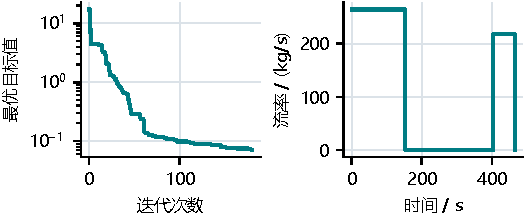
\includegraphics[width=\linewidth,height=42mm]{images/planning_zh.pdf}
\smallnote{左：PSO 最优目标值；右：最终参考流率。燃烧/滑行/燃烧约为 153.3 / 250.0 / 62.0 s。最终精度来自 PSO 与局部精修的共同作用。}
\subhead{MPC：测量 → 预测 → QP → 执行首项}
跟踪参考状态 $x^{\rm ref}=(r,\theta,u,w,m)^\mathsf T$，控制量为偏角与流率修正。沿参考离散线性化后：
\[
 e_{k+1}=A_ke_k+B_kv_k+d_k.
\]

\subhead{滚动时域代价与约束}
\[
\begin{aligned}
 J_{\rm MPC}={}&\sum_{j=1}^{N}\|e_{k+j|k}\|_{Q_j}^2
 +\sum_{j=0}^{N-1}\|v_{k+j|k}\|_R^2\\
 &+\sum_{j=0}^{N-1}\|\Delta v_{k+j|k}\|_{R_\Delta}^2
 +\lambda\|\epsilon\|^2.
\end{aligned}
\]
$e$ 与 $v$ 按物理尺度进行归一化。地面高度用软约束，干质量及输入边界这类高惩罚项采用硬约束。

预测误差、控制幅值、变化率及松弛量的二次代价，经状态消元转化为凸二次规划问题：
\[
 \min_\zeta\ \tfrac12\zeta^\mathsf TH\zeta+f^\mathsf T\zeta,
 \qquad G\zeta\le b.
\]
\textbf{QP 使用凸内点法}，处理偏角、流率、干质量及地面约束。每次仅执行首个修正，再反馈求解；保留原两段燃烧时序。

\subhead{为什么是凸 QP？}
状态消元后，$H=2(\mathcal B^\mathsf T\bar Q\mathcal B+\bar R+D^\mathsf T\bar R_\Delta D)$；正定输入权重使其正定。凸内点法求解扰动 KKT 条件，并逐步减小障碍参数，逼近约束最优解。

\takeaway{离线规划提供可行参考，在线 MPC 补偿受扰动后的状态偏差}
\columnend\colsep
\columnstart
\sect{03}{600 km 算例与结果}
\smallnote{$m_0=60\,000$ kg，$m_{\rm dry}=1\,200$ kg，$c=4\,500$ m/s。开环与闭环使用相同实际扰动；该扰动样本与规划样本不同。}
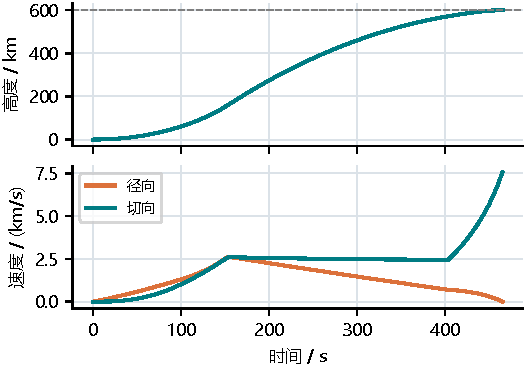
\includegraphics[width=\linewidth,height=60mm]{images/reference_zh.pdf}
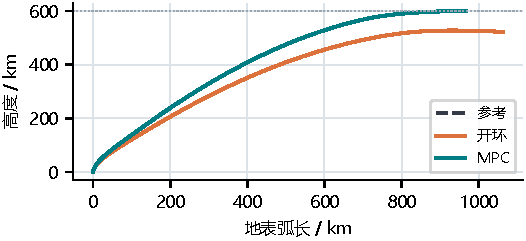
\includegraphics[width=\linewidth,height=48mm]{images/trajectory_zh.pdf}
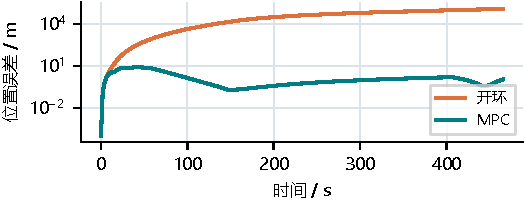
\includegraphics[width=\linewidth,height=40mm]{images/error_zh.pdf}
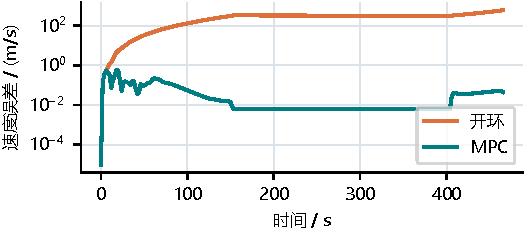
\includegraphics[width=\linewidth,height=40mm]{images/velocity_zh.pdf}
\smallnote{MPC 与参考轨迹在上图基本重合。位置误差为径向误差与地表弧长误差的合成；对数图的零值仅为绘图设置下限。}
\vspace{2pt}
{\fontsize{9.2}{12}\selectfont
\setlength{\tabcolsep}{3pt}
\begin{tabular*}{\linewidth}{@{\extracolsep{\fill}}lrr@{}}
\toprule
指标 & 开环 & MPC\\\midrule
位置跟踪 RMS / m & $5.98\times10^4$ & $2.606$\\
速度跟踪 RMS / (m/s) & $298.084$ & $0.0992$\\
关机高度误差 / m & $-77\,611.6$ & $1.191$\\
关机径向速度 / (m/s) & $-557.983$ & $0.0231$\\
切向速度误差 / (m/s) & $233.256$ & $0.0559$\\\bottomrule
\end{tabular*}}
\smallnote{RMS 相对参考轨迹；关机误差相对目标圆轨道。}
\extrablock{阶段解释与在线求解}
第一段建立上升与横向速度，滑行抬升高度，第二段提高切向速度并压低径向速度。参考关机高度误差为 $0.265$ m，径向与切向速度残差为 $-0.0212$、$0.0463$ m/s。
MPC 每 2 s 更新，预测 30 s；本次 230 次 QP 均成功，平均求解约 1.793 ms。

\takeaway{反馈显著抑制误差积累，终端状态接近目标圆轨道。}

\columnend
\posterfooter{参考：Tsiolkovsky 火箭方程（NASA Glenn）；Kennedy \& Eberhart, Particle Swarm Optimization, 1995；Dormand \& Prince, JCAM, 1980；Mayne et al., Automatica, 2000；Nocedal \& Wright, Numerical Optimization, 2006。\quad 数据：本项目 2026-10-20 冻结实验快照。}
\end{document}
